\chapter{Prevádzka a bezpečnosť sietí}
\phantomsection
Prevádzka sieťových zariadení je proces nielen o~monitorovaní incidentov, zabezpečovaní konzistencie a konvergencie siete, ale aj o~aktualizáciách softvéru a hardvéru, aplikovaní bezpečnostných zásad a politík. Táto kapitola preto opisuje jednotlivé aspekty s~ktorými sa pri prevádzke siete môžeme stretnúť.

\section{Sieťové prvky}
\label{hierarchicky-model}
Medzi základné stavebné piliere sietí, bez ktorých nie je možná komunikácia koncových staníc patria smerovače (router) a prepínače (switch). Mimo týchto dvoch základných zariadení sa v~\zkratka{zkLAN} sieťach často vyskytujú prístupové body (access point), firewally, sieťové mosty (bridge) a v~dnes už ojedinelých prípadoch ešte aj rozbočovače (hub). V~súčasnosti však jedno zariadenie môže kombinovať funkcie zariadení, ktoré majú podľa modelov TCP/IP alebo ISO/OSI na starosti inú vrstvu modelu. Preto sa dnes hlavne z~finančných dôvodov používajú takzvané L3 prepínače, ktoré s~určitými obmedzeniami vedia nahradiť nákladné smerovače. Taktiež smerovače ako aj L3 prepínače umožňujú filtrovanie paketov, takže vedia čiastočne zastať aj základné funkcie firewallu. Značky najpoužívanejších sieťových zariadení sú vyobrazené na obrázku \ref{fig:net-devices} a budú používané v~nasledujúcich kapitolách.

\begin{figure}[H]
	\begin{center}
		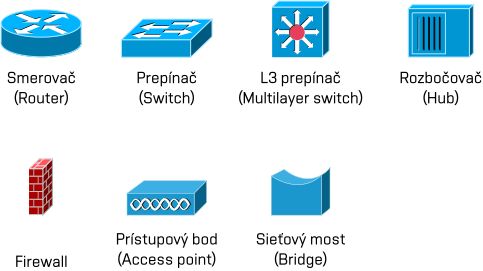
\includegraphics[scale=1.2]{obrazky/net_devices.pdf}
	\end{center}
	\caption[Typy sieťových zariadení v~lokálnych sieťach]{Typy sieťových zariadení v~lokálnych sieťach}
	\label{fig:net-devices}
\end{figure} 

\section{Hierarchický model sietí}
%TODO EDGE
S~postupným nárastom sieťových zariadení a komplexnosti siete dochádza v~sieťach bez hierarchie k~mnohým problémom ako veľké broadcast domény, vysoká cena za port, vysoké zaťaženia zariadení, neprítomnosť redundancie. Preto sa zaviedol hierarchický model siete, ktorý rieši problémy veľkosti a rozsahu broadcast a kolíznych domén, umožňuje efektívne prideľovanie \zkratka{zkIP} adries a oddeľuje zariadenia pracujúce na jednotlivých vrstvách ISO/OSI.  
\\\\
\noindent
Siete sú spravidla delené do 3 vrstiev s~definovanými funkciami \cite{Lammle2013}:
\begin{itemize}
	\item Core\,--\,tvorí vysokorýchlostnú chrbticu siete, agreguje dáta z~distribučnej vrstvy a mala by byť redundantná. Nároky na rýchlosť portov a výkon zariadenia sú obzvlášť vysoké, a preto sa využívajú prevažne smerovače, ale taktiež ako v~distribučnej vrstve dnes už aj L3 prepínače.
	\item Distribučná (Distribution)\,--\,agreguje dáta z~prístupovej vrstvy, vytvára a oddeľuje broadcast domény, riadi smerovanie medzi \zkratka{zkVLAN} a  filtrovanie paketov. Táto vrstva kvôli zabezpečeniu dostupnosti využíva agregovanie  a redundanciu liniek. Typicky sa skladá zo smerovačov, no v~dnešnej dobe hlavne z~L3 prepínačov, keďže tie nie sú finančne také náročné. 
	\item Prístupová (Access)\,--\,vstupný bod do siete, ktorý riadi prístup a politiku pre koncové zariadenia, segmentuje sieť, vytvára a separuje kolízne domény. V~neposlednej rade zariaďujú prístup k~distribučnej vrstve. Je tvorená zariadeniami ako prepínač, rozbočovač alebo prístupový bod.
\end{itemize} 
\vspace{2em}
\begin{figure}[H]
	\begin{center}
		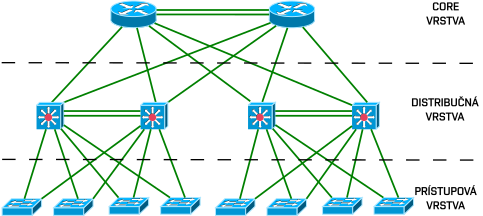
\includegraphics[scale=0.9]{obrazky/hierarchy_network.pdf}
	\end{center}

	\caption[Hierarchické rozdelenie siete na vrstvy]{Hierarchické rozdelenie siete na vrstvy}
	\label{fig:net-hierarchy}
\end{figure} 

\noindent
\vspace{2em}
V~menších sieťach prevažne malých firiem sa využíva zlučovanie vrstiev nazývaných ako collapsed core, ktoré zlučujú distribučnú a core vrstvu, prípadne zlučujú všetky tri vrstvy dokopy. 

\noindent
Cieľom hierarchického modelu a dobre navrhnutej siete je dosiahnutie nasledujúcich vlastností:

\begin{itemize}
	\item Škálovateľnosť\,--\,jednoduché a bezproblémové pridanie zariadenia pri raste a rozširovaní siete.
	\item Redundancia\,--\,zabezpečenie vysokej dostupnosti viacnásobnými linkami medzi zariadeniami a zálohovanie samotných zariadení ich redundanciou.
	\item Výkonnosť\,--\,agregovanie liniek a výber dostatočne výkonných zariadení
	\item Bezpečnosť\,--\,zabezpečenie siete na viacerých úrovniach ako napríklad portoch, oddelením segmentov pomocou VLAN, riadením prístupu, šifrovaním a pod.
	\item Manažovateľnosť\,--\,vytvorenie šablón, definovaných štandardov a pravidiel na zaistenie konzistentnosti konfigurácií zariadení na jednoduchšie odhaľovanie chýb. 
	\item Udržovateľnosť\,--\,schopnosť systému prechádzať zmenami komponentov, služieb a vlastností.
\end{itemize}



\section{Funkčné roviny sieťových prvkov}
Sieťové prvky sú zodpovedné nielen za preposielanie dát medzi koncovými stanicami, ale aj za mnohé riadiace dáta medzi sebou, bez ktorých by sieť nebola funkčná. Preto sa jednotlivé protokoly a služby rozdeľujú troch rovín, a to management, control a data plane. Tieto pojmy sa využívajú vo väčšej miere v~softvérovo definovaných sieťach, no sú platné aj v~klasickej koncepcii.
 
Rovina management je zodpovedná za konfiguráciu a správu zariadení a riadenie prístupu ku konfiguráciám. Typickými príkladmi protokolov pracujúcich na tejto rovine sú \zkratka{zkSNMP}, \zkratka{zkAAA}, Syslog, \zkratka{zkSSH} a mnohé ďalšie \cite{Singh2018}. Druhá rovina, control plane má na starosti prevažne riadenie siete a smerovanie. Zaoberá sa otázkou kadiaľ budú pakety smerované a prenáša riadiace a signalizačné informácie pre protokoly ako napríklad, \zkratka{zkOSPF}, Spanning tree, \zk{zkFHRP} \cite{Singh2018}. Poslednou rovina je data plane nazývaná často aj forwarding plane, ktorá prepína pakety na daný port na základe rozhodnutia z~control plane. Táto časť sieťových prvkov musí byť veľmi rýchla, aby zaistila nízku odozvu a dostatočne vysoké prenosové rýchlosti. Nižšie uvedený obrázok \ref{fig:sdn-planes} reflektuje tok dát z~jednej roviny do druhej a tiež medzi dvoma susednými zariadeniami. Rovina management plane zodpovedná za konfiguráciu zariadenia a nastavuje rovina control plane, v~tomto prípade smerovanie z~zariadení. Po výmene informácií so susednými smerovačmi sa vytvoria príslušné tabuľky a nakoniec smerovacia tabuľka, ktorá sa využíva pri rozhodovaní prepínania paketov v~rovine data plane.

\begin{figure}[H]
	\begin{center}
		\includegraphics[scale=0.6]{obrazky/SDN_planes.pdf}
	\end{center}
	\caption[Rozdelenie rovín v~smerovači, tok informácií v~jeho vnútri a medzi susednými smerovačmi]{Rozdelenie rovín v~smerovači, tok informácií v~jeho vnútri a medzi susednými smerovačmi \cite{Pepelnjak2013}}
	\label{fig:sdn-planes}
\end{figure} 


\section{Prevádzkové a bezpečnostné postupy}

\subsection{Riadenie a zneužitie prístupu k~manažmentu zariadenia}
Kritickým miestom často absentujúcim zabezpečenie je prístup ku konfigurácií zariadenia. Typickým príkladom je využitie protokolu Telnet, ktorý nešifruje spojenie a je teda ľahko odpočúvateľný. Preto sa odporúča využívať protokol \zk{zkSSH}, naviac je dobré využiť bezpečnú verziu 2 s~rozumnou dĺžkou kľúča odpovedajúcou aktuálnym odporúčaniam \cite{CIS_DrTLsgXv24lxeIIM} \cite{Barker2019}. Jedným z~opatrení na zabezpečenie SSH prístupu je zmena portu, na ktorom obvykle počúva z~dôvodu, že útočník skúša periodicky útoky hrubou silou na \zkratka{zkTCP} port 22. Alternatívou na zabezpečenie SSH prístupu môže byť port knocking, ktorý na základe autorizácie dynamicky povolí záznam v~ACL k~portu, na ktorom počúva SSH.

Pri pokusoch o~prihlásenie sa často využíva hádanie hesiel, preto je dobré určiť maximálny počet neúspešných pokusov a definovať čas po ktorý bude prihlásenie zablokované.

Riadenie prístupu k~manažmentu zariadení by malo byť výhradne z~obmedzeného rozsahu staníc administrátorov, na to poslúžia obmedzenia pomocou \zk{zkACL}, aby neprišlo k~nechcenému prihláseniu alebo útoku \zk{zkDoS} z~nechcených klientský staníc. Je tiež dobré zaznamenávať neúspešné ale aj úspešné prihlásenia do manažmentu zariadenia. 

V~prípade konfigurácie viacerými administrátormi naraz môže vzniknúť konflikt, a preto je dobré zabezpečiť, aby v~jednom okamihu mohol zmeny vykonávať iba jeden administrátor. Problémom môžu byť aj dlhé aktívne pripojenie k~manažmentu zariadenia, ktoré môže byť zneužité pri odblokovanom počítači administrátora. 

Pri pokuse o~prihlásenie alebo zmene nastavení je dobré informovať oznámením alebo správou potenciálneho útočníka s~následkami, ktoré mu hrozia v~prípade zneužitia zariadenia \cite{CIS_DrTLsgXv24lxeIIM}. 

\begin{figure}[H]
	\begin{center}
		\includegraphics[scale=1]{obrazky/login-log.pdf}
	\end{center}
	\caption[Prihlasovanie k~manažmentu zariadenia z~povolených IP adries a logovanie pokusov z~nepovolených IP adries]{Prihlasovanie k~manažmentu zariadenia z~povolených IP adries a logovanie pokusov z~nepovolených IP adries}
	\label{fig:login-log-mngmt}
\end{figure} 

\newpage
Ďalšou obranou proti nechcenému prístupu na sieťové prvky je vytvorenie lokálnych účtov, ktoré budú použité na prihlasovanie a pri zmenách konfigurácie. Bez znalosti kombinácií mena a hesla by nemalo byť umožnené zmeniť nastavenia zariadenia.  

\subsubsection{Riadenie prístupu pomocou AAA}
Najlepším riešením pre riadenie prístupu k~manažmentu zariadenia a účtovaniu sú protokoly spadajúce do skupiny \zk{zkAAA}. Patria sem protokoly \texttt{Radius}, \texttt{TACACS+} alebo \texttt{Kerberos}. Tieto protokoly umožňujú okrem riadenia prihlásení administrátorov taktiež špecifikovať príkazy konfigurácie, ktoré budú jednotlivcom povolené a tiež zaznamenávať zmeny jednotlivých administrátorov v~konfigurácií, ktoré učinili a naviac aj kedy boli na zariadení prihlásení. Zároveň je treba určiť aj mechanizmus prihlásenia pri výpadku autentifikačného serveru, teda napríklad nejaké záložné lokálne konto.

\begin{figure}[H]
	\begin{center}
		\includegraphics[scale=1.1]{obrazky/AAA.pdf}
	\end{center}
	\caption[Overenie prihlásenia k~manažmentu zariadenia pomocou AAA serveru]{Overenie prihlásenia k~manažmentu zariadenia pomocou AAA serveru}
	\label{fig:aaa-mngmt}
\end{figure} 



\subsection{Filtrovanie prevádzky}
Filtrovanie prevádzky môže prebiehať pomocou ACL, teda súborom pravidiel na vrstve L3 a L4, ktoré povoľujú alebo zakazujú komunikáciu. Jedným z~dobrých praktík je filtrovať pakety so zdrojovou adresou privátnych alebo špeciálnych adries v~smere do vnútornej siete z~internetu \cite{Jackson2010}. Rozsahy týchto IP adries sú definované v~RFC 6890 \cite{rfc6890al6BqxiLuoAdpLeG} a v~RFC 8190 \cite{rfc8190O1cp1uhrCiYj0LYK}. Administrátori často zabúdajú pri implementácií IPv6, že aj tento protokol má špeciálne adresy, ktoré nemôžu byť zdrojové, ak paket prichádza z~internetu. Špeciálne IPv6 adresy sú definované v~RFC 5156 \cite{rfc5156lPYdBFaqWC5RwyJI} a aj vo vyššie spomenutých RFC. V~prípade použitia týchto špeciálnych adries ako zdrojových sa jedná o~útok typu IP spoofing.

\subsubsection{IP Options}
Protokol IPv4 umožňuje pomocou poľa Options vynútenie smerovania na základe zdrojovej adresy a definovanie cesty paketu, ale aj mnohé iné funkcionality. Toto pole nie je však používané a odporúča sa zahadzovať pakety obsahujúce pole Options \cite{Singh2018}. Jedným z~dôvodov je preťaženie smerovača, keďže každý paket sa musí spracovávať v~procesore a nemôže byť akcelerovaný v~špeciálnych obvodoch a tým urýchlené jeho preposlanie. 

\subsubsection{IPv6 rozšírené hlavičky}
Protokol IPv6 nemá pole Options, ale tzv. Next Header. Problémom s~rozšírenou hlavičkou sa zaoberá v~článkoch Martin Grégr a Tomáš Podermański \cite{Gregr2622015} \cite{Podermanski1922015}. V~tomto poli môže byť definovaný protokol vyššej vrstvy, napríklad TCP, ale aj rozšírená hlavička, preto má smerovač problém často rozpoznať, ktoré z~týchto dvoch sa nachádza v~políčku a ako sa má zachovať, či ide o~rozšírenú hlavičku alebo nový protokol. To čo nastane s~paketom a ako sa zariadenie zachová závisí od implementácie softvéru v~smerovači. Ten sa môže reštartovať, hlavičku preskočiť, zahodiť paket alebo na základe nesprávneho spracovania preskočiť pravidlo zahodenia paketu. Z~týchto dôvodov a hlavne preskočením filtrácie sú rozširujúce hlavičky nebezpečné. Administrátor sa môže k~ním stavať viacerými spôsobmi, a to zahodením každého paketu s~rozširujúcou hlavičkou, zahodenie paketu s~neznámou hlavičkou alebo ignorovanie tohto problému. Keďže niektoré rozširujúce hlavičky sú potrebné a používané, tak je dobrou zásadou odfiltrovať práve tie, ktoré zariadenie nevie rozpoznať. V~súvislosti s~rozšírenými hlavičkami sa zneužíva aj fragmentácia, a to takým spôsobom, že paket sa rozdelí na malé časti a rozšírená hlavička je až v~poslednom fragmentovanom pakete. Predpokladá sa, že zariadenie si nevie znovu poskladať a spracovať takto zreťazenú hlavičku a preto dôjde k~obídeniu filtrovacích pravidiel. Touto problematikou sa zaoberá RFC 7112, ktoré definuje, aby rozšírená hlavička bola už v~prvom pakete a tým bolo možné rozpoznať o~akú rozšírenú hlavičku ide. Plošné zakázanie rozširujúcich hlavičiek nie je dobré, keďže sa využíva aj pre IPSec.

\subsection{Smerovacie protokoly}
%TODO virtual link, auto summary
Používaním dynamických smerovacích protokolov prichádza sieť o~určitú časť bezpečnosti a to vysielaním informácií o~pripojených a naučených sieťach a cestách, ktoré môže útočník odchytávať. K~tomu sa ešte môže pridať vloženie falošnej informácie a teda zaistenie smerovania cez útočníka. Našťastie obrana proti týmto útokom existuje, aj keď nie je vždy ideálna. V~prípade vloženia informácie alebo cesty do správ, ktoré si vymieňajú dynamické smerovacie protokoly je možnou obranou autentifikácia správ poslaných medzi smerovačmi \cite{McMillan2018} \cite{Singh2018} \cite{CIS_DrTLsgXv24lxeIIM}. Pri zasielaní sa používa hash hesla a to sa pri prijatí druhým smerovačom porovná s~vopred definovaným. Na obrázku \ref{fig:passive-int} je vidno, že informácie dynamického smerovacieho protokolu sú zastavené na pasívnom rozhraní \cite{Khandelwal2016}, a teda užívatelia alebo útočník nemá možnosť sa tieto údaje dozvedieť.

\begin{figure}[H]
	\begin{center}
		\includegraphics[scale=1]{obrazky/passive-interface.pdf}
	\end{center}
	\caption[Blokovanie správ dynamického smerovacieho protokolu na pasívne rozhranie]{Blokovanie správ dynamického smerovacieho protokolu na pasívne rozhranie}
	\label{fig:passive-int}
\end{figure} 

\subsubsection{Source Routing}
Bezpečnostnou hrozbou môže byť aj smerovanie na základe zdrojové adresy, pri ktorej si zdroj určí cestu, ktorou bude paket prechádzať namiesto aby túto skutočnosť prenechal na rozhodnutí smerovačov po ceste k~cieľu \cite{CIS_DrTLsgXv24lxeIIM}. Táto funkcia využíva pole \texttt{IP Options}, ktoré býva však často ignorované prípadne pakety s~týmto polom zahadzované z~bezpečnostných dôvodov. Existujú dva módy, a to Strict a Loose, v~prvom prípade musí paket prejsť všetkými definovanými bodmi a žiadnym iným. Naopak mód Loose definuje uzly ,ktoré je potreba navštíviť, no zároveň môžu byť navštívené aj iné uzly po ceste.  

\subsubsection{Unicast reverse path forwarding}
Podvrhnutie IP adresy, tzv. IP spoofing je jedným z~útokov, ktorým musia smerovače čeliť. Dá sa mu zbrániť pomocou \zkratka{zkURPF} \cite{Jackson2010}, ktorý funguje buď v~Strict alebo Loose móde a zisťuje prítomnosť zdrojovej zdrojovej IP adresy. Ako už názov napovedá, tak mód Strict je prísnejší, pretože zahadzuje pakety, ktorej zdrojová adresa sa nenachádza v~smerovacej tabuľke a zároveň testuje či zdrojová adresa je dosiahnuteľná cez rozhranie, na ktorom bol paket prijatý. Tento mód je preto nevhodný pri asymetrickom smerovaní. Mód Loose testuje prítomnosť zdrojovej adresy iba v~smerovacej tabuľke. 

\subsubsection{BGP TTL Security}
Protokol \zkratka{zkBGP} okrem autentifikácie obsahuje aj ďalšiu ochranu a to \zkratka{zkTTL} security \cite{AlHFaPbj6IbKzbuv}. Pri tomto prístupe sa porovnáva hodnota poľa TTL v~pakete, ktorý dorazí do smerovača a známy počet skokov, ktorý sa nakonfiguruje medzi našim smerovačom a zdrojom. Mohlo by sa zdať, že priamo pripojené siete, teda susedné autonómne systémy týmto problémom netrpia, no pole TTL sa dá zmeniť tak, aby po príchode na smerovač obete malo toto pole hodnotu 1, čo je predvolené TTL, ktoré zasiela BGP, viď obrázok \ref{fig:ttl-sec}. Z~tohto dôvodu sa používa obrátená forma kontroly, a to testovanie voči maximálnej hodnote TTL, čo je hodnota 255. To znamená, že všetky pakety od priamo pripojených BGP susedov budú mať po príchode na náš smerovač hodnotu TTL 255, tie ktoré to nebudú splňovať sú brané ako nelegitímne pakety, viď \ref{fig:ttl-sec}. Treba dodať, že v~prípade že smerovače nie sú priamo pripojené, tak je možné použiť aj definovanie vzdialenosti medzi smerovačmi, teda počet skokov, aby susedný smerovač dostal BGP správu. Bezpečnejšie je však použiť TTL security, tak že sa od čísla 255 odpočíta počet skokov medzi dvoma autonómnymi systémami a voči tejto hodnote sa bude robiť kontrola.

\begin{figure}[H]
	\begin{center}
		\includegraphics[scale=1]{obrazky/ttl-sec.pdf}
	\end{center}
	\caption[Porovnanie prístupov TTL security]{Porovnanie prístupov TTL security, kde sa v~prvom prípade používa implicitná hodnota 1 na porovnanie TTL a v~druhom prípade maximálna hodnota TTL \cite{AlHFaPbj6IbKzbuv}}
	\label{fig:ttl-sec}
\end{figure} 


\subsection{Identifikácia zariadení, pravidiel a nastavení}
K~lepšej identifikácií je dobrým pravidlom každé sieťové zariadenie vhodne pomenovať kombináciou typu zariadenie, vrstvy hierarchického modelu, na ktorej operuje a prípadne umiestnenia v~racku, napríklad \texttt{sw01-dist-rack1}. V~súvislosti s~týmto nastavením sa často nastavuje aj doména, v~ktorej je zariadenie umiestnené. Tieto dve prerekvizity potom umožňujú aj vzdialenú správu zariadenia a prístup cez SSH \cite{CIS_DrTLsgXv24lxeIIM}.

Dôležitým prvkom sú komentáre k~pravidlám v~\zk{zkACL}, ktoré by mali nielen identifikovať, čo presne dané pravidlo povoľuje a zakazuje, ale aj identifikovať požiadavok, na základe ktorého bolo pravidlo vytvorené. 

Komentáre s~popisom je dobré pridávať aj na rozhrania sieťových zariadení, napríklad s~popisom, k~akému zariadeniu dané rozhranie vedie. Posledným, ale nemenej dôležitým je pomenovanie \zk{zkVLAN} pre ich ľahšiu identifikáciu.

\subsection{Šifrovanie hesiel}
Pri úniku konfigurácií môže dôjsť k~odhaleniu hesiel uložených v~nich, preto by mali byť v~konfiguračnom súbore všetky heslá zahašované pomocou čo najpokročilejších hašovacích funkcií, ktoré dané zariadenie podporuje \cite{CIS_DrTLsgXv24lxeIIM}.

\subsection{Logovanie}
Záznam činnosti zariadenia patrí k~základným prvkom monitorovania sieťovej infraštruktúry spolu s~notifikovaním o~vzniknutých incidentoch. Na tieto účely sa používa prevažne dva protokoly, a to \zkratka{zkSNMP} a Syslog. 

Protokol SNMP využíva databázu MIB buď štandardizovanú, alebo rozšírenú daným výrobcom zariadenia. Jednotlivé monitorované objekty sú v~tejto databáze organizované v~stromovej štruktúre. V~súčasnosti sa využívajú prevažne SNMP verzie 2c a 3. Je vysoko odporúčané využívať verziu 3, ktorá zabezpečuje ako integritu, tak aj dôvernosť a autentifikáciu \cite{CIS_DrTLsgXv24lxeIIM} \cite{Graesser2001}. Protokol SNMP umožňuje pomocou jednotlivých objektov meniť nastavenia zariadení, túto funkciu je však dobré vypnúť a povoliť iba čítanie objektov z~presne definovaných IP adries pomocou ACL a asynchrónne správy TRAP.   

Druhou možnosťou monitorovania a notifikovania o~incidentoch je protokol Syslog. Typicky sa nastavuje Syslog server, ktorý zbiera správy z~viacerých zariadení, ktoré môžu byť následne spracovávané špeciálnymi programami a vizualizované v~dohľadových centrách. Protokol Syslog pozná 8 úrovní dôležitosti (severity), pričom čím nižšie číslo dôležitosti, tým ide o~závažnejší problém. Pri výpadku Syslog serveru je nutné záznamy ponechať na zariadení a preto mať dostatočné množstvo pamäte \cite{Singh2018} \cite{uYLsMtQInofenpV3}. V~niektorých prípadoch môžu zariadenia vygenerovať väčšie množstvo správ, ktoré majú rovnaký čas a z~tohto dôvodu by mali mať jednotlivé správy s~rovnakým časom vzniku jednoznačné sekvenčné číslo, aby bolo možné zistiť postupnosť, v~akom vznikli incidenty, napríklad zmeny v~susedstvách dynamických smerovacích protokoloch.

Veľa útokov mieri práve na protokol SNMP, a preto ho mnohí odporúčajú vypínať \cite{CIS_DrTLsgXv24lxeIIM}, na druhej strane protokol Syslog nezabezpečuje žiadnu časť z~triády CIA.   


\subsection{Synchronizácia času}
Správny a aktuálny čas je dôležitý hlavne pre správne fungovanie certifikátov a protokolu Syslog. V~prípade protokolu Syslog zabezpečuje jednoznačnú identifikáciu incidentu v~správnom čase a teda lepšiu dohľadatelnosť a určenie vzniku problému. Keďže tento protokol využíva \zkratka{zkUDP}, tak je náchylný na DDoS reflektívne amplifikačné útoky. Tento typ útoku využíva krátku správu zasielanú na NTP server s~podvrhnutou zdrojovou IP adresou (IP Spoofing), na ktorú budú zasielané odpovede s~oveľa väčšou veľkosťou ako boli pôvodné správy na NTP server. Bohužiaľ obrana proti tomuto typu útoku je veľmi ťažká, poskytovatelia pripojenia k~internetu sa s~týmto neduhom väčšinou dokážu popasovať \cite{gTkmbyKon9H6tuAm}, v~lokálnych sieťach môže pomôcť IP Snooping. Podľa Network Time Foundation \cite{s0goWNnWp5OjqREE}, aktuálna verzia protokolu 4 nepodporuje šifrovanie správ, no poskytuje akú-takú bezpečnosť pre koncových NTP klientov pomocou MD5 a to autentifikáciu NTP serveru a kontrolu integrity. Naviac protokol nepodporuje žiadnu distribúciu kľúčov. Protokol NTP verzie 4 podporuje aj asymetrickú kryptografiu pomocou Autokey, no podpora tohto riešenia je veľmi slabá \cite{s0goWNnWp5OjqREE}, jedným z~dôvodov je aj náročnosť výpočtov. NTP podporuje sťahovanie správ aj od klientov, toto je výhodné pri prerušení linky ku NTP serveru a na krížovú kontrolu času. Dôležitým nastavením je aj správne časové pásmo, ktoré je dobré zjednotiť naprieč všetkými spravovanými zariadeniami. V~prípade roztrúsenia zariadení cez viacero časových pásiem je dobré využívať univerzálny čas UTC. Okrem protokolu NTP existuje niekoľko ďalších protokolov na synchronizáciu času, no sú menej používané. Príkladom je \zkratka{zkPTP}, ktorý je vhodný do lokálnych sietí kvôli vysokej presnosti. 

\begin{figure}[H]
	\begin{center}
		\includegraphics[scale=0.75]{obrazky/ntp_amplification.pdf}
	\end{center}
	\caption[Ilustrácia amplifikačného útoku cez nakazený počítač pomocou podvrhnutej IP adresy]{Ilustrácia amplifikačného útoku cez nakazený počítač pomocou podvrhnutej IP adresy \cite{gTkmbyKon9H6tuAm}}
	\label{fig:ntp-amp}
\end{figure} 

\subsection{Záloha a zabezpečenie konfigurácií}
Konfigurácie zariadení a ich záloha sú veľmi dôležitým faktorom, ktorým sa treba zaoberať pri správe infraštruktúry. Pokiaľ sú prítomné aktuálne konfigurácie zariadení, tak pri výpadku hardware je možné ho vymeniť za nový a aplikovať fungujúcu konfiguráciu z~poškodeného zariadenia zo zálohy. Zároveň by sa konfigurácia mala dostatočne zabezpečiť proti výmazu zo zariadenia a zálohovaného úložiska a dostatočne zabezpečiť \cite{McMillan2018}. Zabezpečenie je dôležité, aby nedošlo k~úniku konfigurácie útočníkom a nepovolaným osobám a následnému zneužitiu. Záloha konfigurácií by sa mala robiť cez zabezpečený kanál najlepšie pomocou protokolov podporujúcich šifrovanie, napríklad \zkratka{zkSCP} alebo \zkratka{zkSFTP} a nie pomocou \zkratka{zkTFTP} \cite{Singh2018}. Vhodná je aj prítomnosť záznamu zmien v~konfigurácií v~čase \cite{McMillan2018}.

\subsection{Správanie pri vysokom zaťažení}
V~priebehu prevádzky sa môže vyskytnúť kratší alebo aj dlhý časový okamih, kedy je zariadenie vysoko zaťažené a nezvláda spracovávať požiadavky. Toto môže byť spôsobené útokom (D)DOS alebo nedostatočným dimenzovaním a zlou architektúrou siete. Aj napriek tomuto stavu by však malo byť zariadenie schopné odosielať chybové správy a notifikovať o~problémoch. Zároveň by mali byť nastavené prahové hodnoty, ktoré budú indikovať stav, že môže dôjsť k~nadmernému vyťaženiu procesoru, pamäti alebo linky či už pomocou Syslog správ alebo protokolu SNMP \cite{uYLsMtQInofenpV3} \cite{Singh2018}.

\subsection{Monitorovanie výkonu siete}
Monitorovanie siete nie je len o~chybových a operačných správach zariadení, ale aj o~prevádzke, ktorá v~sieti prebieha. Toto monitorovanie prevádzky musí byť vykonávané často z~legislatívnych dôvodov a aplikuje sa u~poskytovateľov pripojenia. Monitorovanie prevádzky sa však vykonáva aj v~lokálnych sieťach, napríklad zrkadlením portov \cite{Singh2018} na analýzu útokov pre IDS alebo pre štatistické informácie a informácie o~zaťažení pomocou protokolov sFlow a NetFlow.

\subsection{Problémy vrstvy L2}
Prístupová vrstva hierarchického modelu alebo vrstva L2 modelu ISO/OSI je časť siete, do ktorej sa pripájajú zväčša koncové zariadenia. Vzniká tu preto mnoho problémov či už bezpečnostných alebo prevádzkových, na ktoré je nutné myslieť.

\subsubsection{Spanning Tree Protocol}
Protokolom pracujúcim na vrstve L2 je \zkratka{zkSTP}, zaisťujúci bezslučkovú topológiu aj v~prípade cyklického zapojenia prepínačov z~dôvodu redundancie \cite{Lammle2013}. Existuje mnoho implementácií STP protokolu, každé však zabezpečuje logické vypnutie alebo zakázanie portu aj pri existujúcom fyzickom pripojení. Pre urýchlenie výpočtu kostry a konvergencie siete sa vylučujú z~výpočtu porty, na ktoré sú pripojené koncové zariadenia a teda nepredpokladá sa na týchto portoch pripojený prepínač. Tento fakt môže na druhej strane spôsobiť slučky v~prípade zapojenie prepínača do takéhoto portu. Z~tohto dôvodu existuje tzv. BPDU Guard \cite{Lammle2013}, čo je ochrana, kedy pri prijatí rámca s~BPDU označeným červeno na obrázku  \ref{fig:bpdu-guard} na port vyradený z~výpočtu kostry grafu je port zablokovaný a neumožňuje preposielať rámce. Ďalšou ochranou je Root Guard \cite{Vyncke2008}, ktorý zabraňuje novo pripojeným prepínačom prebrať rolu hlavného prepínača pre danú podsieť alebo VLAN. Jeho úžitok zobrazuje nasledujúci obrázok \ref{fig:root-guard}, kde po pripojení nedovoleného prepínača označeného červeno príde nepríde k~zvoleniu nového Root Bridge kvôli ochrane Root Guard. Existuje ešte ochrana Loop Guard \cite{Vyncke2008}, ktorá zabezpečuje, že pri poruche a jednosmernej komunikácií medzi prepínačmi nedôjde k~vytvoreniu slučiek. Táto ochrana je však výhradne u~zariadení od spoločnosti Cisco. 

\begin{figure}[H]
	\begin{center}
		\includegraphics[scale=0.75]{obrazky/root-guard.pdf}
	\end{center}
	\caption[Zabránenie prebratia role Root Bridge pomocou Root Guard]{Zabránenie prebratia role Root Bridge pomocou Root Guard, kde pri pripojení nedovoleného prepínača (označený červeno) s~nižšou MAC adresou nebude prepínač zvolený za Root Bridge}
	\label{fig:root-guard}
\end{figure} 

\begin{figure}[H]
	\begin{center}
		\includegraphics[scale=0.75]{obrazky/bpdu-guard.pdf}
	\end{center}
	\caption[Zabránenie vyhlásenie koncového portu ako portu k~prepínáču pomocou BPDU Guard]{Zabránenie vyhlásenie koncového portu ako portu k~prepínáču pomocou BPDU Guard, kde po prijatí rámcu s~BPDU označeným červeno, príde k~zablokovaniu portu}
	\label{fig:bpdu-guard}
\end{figure} 

\subsubsection{Bezpečnosť VLAN}
Referenčná príručka bezpečnosti \cite{uYLsMtQInofenpV3} definuje nižšie popísané útoky na vrstve L2 a obranu na ne. V~predvolenom stave sú zväčša všetky porty v~jednej VLAN, ktorá je implicitne povolená na všetkých trunk portoch respektíve portoch, kadiaľ prechádza tagovaná prevádzka. Preto je dobré všetky aj nepoužívané porty odobrať z~predvolenej VLAN a nepripojené porty prideliť nikam nesmerovanej VLAN. Taktiež by sa predvolená VLAN nemala používať na tagovanú prevádzku a to aj z~dôvodu, že pri zabudnutí odstránenia prístupových portov z~predvolenej VLAN môže dôjsť k~útokom VLAN hopping za pomoci Double tagging. Na tagovaných trunk portoch by mala byť povolená prevádzka iba takých VLAN, ktoré sú potrebné a zakázaná pre VLAN, do ktorej sú umiestnené nevyužívané porty. Útoku double tagging sa dá zabrániť špecifikovaním VLAN na prístupových portoch a definovaním separátnej VLAN na tagovaných trunk portoch.

\begin{figure}[H]
	\begin{center}
		\includegraphics[scale=0.75]{obrazky/double-tagging.pdf}
	\end{center}
	\caption[VLAN Hopping s~Double Tagging]{Útok Double tagging, pri ktorom útočník zasiela rámec s~dvoma VLAN ID, kde prvé bude odstránené na prvým prepínačom, keďže trunk má tagovanú prevádzku na VLAN 100, tak dôjde k~preposlaniu rámcu až k~obeti \cite{srOo9OPXJxHjPBgo}}
	\label{fig:double-tagging}
\end{figure} 

Predstieranie, že koncové zariadenie je prepínač sa dá zneužitím protokolu \zkratka{zkDTP} \cite{uYLsMtQInofenpV3}. Pri tomto útoku s~názvom Switch spoofing, prepínač aktívne alebo pasívne čaká na odpoveď, že na druhej strane prístupového portu je prepínač. Ak mu dôjde od koncového zariadenia takáto správa, tak sa prepne pôvodne prístupový port na port typu trunk. Z~tohto dôvodu je dobrou zásadou tento protokol nevyužívať a porty konfigurovať ručne ako prístupové alebo trunk.

\begin{figure}[H]
	\begin{center}
		\includegraphics[scale=0.75]{obrazky/switch-spoofing.pdf}
	\end{center}
	\caption[Útok Switch spoofing pomocou protokolu DTP]{Útok Switch spoofing pomocou protokolu DTP, prepínač aktívne čaká na správu DTP alebo stav portu trunk, útočník zasiela správu (označenú červeno) žiadajúcu o~vytvorenie trunk portu, trunk bude nakoniec vytvorený}
	\label{fig:switch-spoofing}
\end{figure} 


Istou formou zabezpečenia je aj explicitne zakázať nepoužívané prístupové porty, aby ich nebolo možné zneužiť, keďže často pri neaktívnych portoch absentujú rôzne bezpečnostné nastavenia, z~dôvodu, že pri prvotnom nasadení zariadenia sa nevyužívali.  

Proprietárny protokol \zkratka{zkVTP} a štandardizovaný \zkratka{zkMVRP} a ich predchodcovia umožňujú distribúciu a synchronizáciu VLAN informácií na skupinu prepínačov \cite{Vyncke2008}. Na jednej strane tieto protokoly uľahčujú administráciu, no pri neopatrnosti môže pri zapojení nového zariadenia do siete prísť k~výmazu VLAN informácií na všetkých pôvodných prepínačoch. Preto je dobré tento protokol používať iba pri prvotnom nasadení a vytváraní siete. V~prípade nutnosti používania tohto protokolu je dobré zabezpečiť správy posielané medzi prepínačmi, aby nedošlo k~ich manipulácií po ceste. Taktiež je v~prípade použitie týchto protokolov výhodné zapnúť funkciu pruning, ktorá umožňuje zasielať broadcast iba na tie prepínače, ktoré majú porty v~danej VLAN. 
%TODO Túto funkciu reprezentuje nasledujúci obrázok \ref{fig:vtp-pruning}


\subsection{First Hop Security}
First Hop Security je označenie pre niekoľko prístupov k~zabezpečeniu koncových staníc a mitigáciu rôznych zneužití a podvrhnutí. Treba povedať, že protokoly IPv4 a IPv6 sa mierne odlišujú vzhľadom ku rozdielnemu postoju k~prideľovaniu adries \cite{Satrapa2019}.

\subsubsection{Port Security}
Prístupové porty, ktoré sa využívajú na pripojenie klientských staníc zväčša absentujú akoukoľvek identifikáciou pripojeného zariadenia. Najjednoduchším spôsobom je definovanie maximálne jednej povolenej MAC adresy na porte. Tento typ obrany naviac zamedzí útoku MAC flooding, kde dochádza k~zaplaveniu portu náhodnými MAC adresami za účelom preťažiť CAM tabuľku prepínača a donútiť ho posielať všetko ako broadcast. Pri prekročení limitu počtu adries na port by mal byť notifikovaný administrátor a port by mal pozastaviť preposielanie rámcov.

Napriek vyššie zmienenému opatreniu, nič nebráni útočníkovi zmeniť MAC adresu na útočiacom zariadení, aby mu bol povolený prístup do lokálnej siete, tento typ zneužitia sa volá MAC spoofing. Naviac takéto nastavenie zamedzí využívanie prípojky legitímnym užívateľom. Z~tohto dôvodu vznikol štandard 802.1x, ktorý definuje akým spôsobom bude užívateľ respektíve koncová stanica na porte autentizovaná \cite{Vyncke2008}. Tento štandard využíva protokoly \zkratka{zkEAP}, \zkratka{zkPEAP}, \zkratka{zkEAPoL}, RADIUS, TACACS+, Kerberos a definuje tri role pre zariadenia podieľajúce sa na autentifikácií. Prvým typom zariadenia je Supplicant, čo je koncové zariadenie , ktoré zasiela prístupové údaje na zariadenie Authenticator, ktorým je zväčša prepínač. Na porte prepínača, na ktorý je pripojený Supplicant sú bez overenia povolené len protokoly EAP, EAPOL prípadne CDP/LLDP a je umiestnený do izolovanej VLAN. Po úspešnom overení pomocou autentifikačného serveru, ktorý porovná preposlané prihlasovacie údaje od prepínača s~autentifikačným serverom, budú no porte povolené všetky potrebné protokoly a koncové zariadenie bude v~náležitej VLAN. Nižšie uvedený zjednodušený obrázok \ref{fig:dot1x} ilustruje komunikáciu koncovej stanice s~prepínačom a autentifikačným serverom.  

\begin{figure}[H]
	\begin{center}
		\includegraphics[scale=0.75]{obrazky/dot1x.pdf}
	\end{center}
	\caption[Autentifikácia 802.1x zjednodušene]{Zjednodušená komunikácia koncovej stanice s~prepínačom, ktorý preposiela prihlasovacie údaje serveru na overenie na následné povolenie komunikácie na porte \cite{Vyncke2008}}
	\label{fig:dot1x}
\end{figure}


\subsubsection{DHCP Snooping}
Protokol IPv4 využíva centralizované prideľovanie IP adries za pomoci DHCP serveru. Výhodou je, že všetky pridelené adresy sú dostupné na jednom mieste, no zároveň toto riešenie porušuje vrstvový model sietí, keďže aplikačný protokol DHCP konfiguruje protokol nižšej vrstvy. Problém v~prípade útoku DHCP spoofing Man-in-the-middle je, že v~sieti môže byť viacero DHCP serverov a ten, ktorý odpovie rýchlejšie, teda útočníkov môže prinútiť koncovú stanicu, aby si vybrala adresu ponúkanú ním. To znamená, že môže napríklad všetku sieťovú prevádzku z~koncového zariadenia smerovať cez bod siete, ktorý útočníkovi vyhovuje. Obranou na tento útok je DHCP snooping \cite{Vyncke2008} \cite{Singh2018}, kedy sa definujú porty, ktoré sú dôveryhodné a teda, môžeme z~nich prijímať správy DHCP Offer a DHCP Acknowledge. Prepínač si následne vytvorí mapovanie IP adresy pridelenej DHCP serverom, MAC adresy koncového zariadenia, VLAN a portu, na ktorom je zariadenie pripojené. DHCP Snooping tiež zabraňuje vyčerpaniu adries pridelených pomocou DHCP serveru, kde útočník posiela správy DHCP Request s~podvrhnutými MAC adresami, aby vyčerpal rozsah, ktorý sa prideľuje klientom.

\subsubsection{Dynamic ARP Inspection}
Protokol ARP býva zneužitý na útok ARP spoofing. Pri tomto útoku útočník na dotaz užívateľa, v~ktorom sa pýta, akú MAC adresu má zariadenie, ku ktorému pozná IP adresu, odpovie svojou MAC adresou alebo MAC adresou uzla v~sieti, cez ktorý má prechádzať komunikácia. Týmto zabezpečí, že dáta bude možné odchytávať na stanici, ku ktorej má prístup. Obranou proti tomuto zneužitiu je Dynamic ARP Inspection \cite{McMillan2018}, ktorá porovnáva údaje získané z~tabuľky vybudovanej pomocou DHCP Snoopingu. Pokiaľ ARP odpoveď z~portu neodpovedá naučenej informácii, tak je paket ARP odpovedi zahodený. Preto je nutnosťou pre využitie tejto obrany mať zapnutú funkciu DHCP snooping.

\subsubsection{IP Source Guard}
Ďalším častým útokom na prístupovej vrstve je IP spoofing, a teda používanie a zneužitie IP adresy, ktorá koncovému zariadeniu nepatrí. Útočník pomocou tohto útoku môže zahltiť stanicu tak, že ako zdrojovú IP adresu paketu uvedie IP adresu obeti a predpokladá, že odpoveď na tento paket už nebude doručená jemu, ale obeti. Mitigácia tohto útoku je možná za pomoci IP Source Guard \cite{Singh2018}, ktorá v~každom odchádzajúcom pakete skontroluje, či IP adresa vysielajúcej stanice súhlasí so zdrojovou IP adresou. Nutnou prerekvizitou je vybudovanie tabuľky za pomoci DHCP snoopingu.    

\begin{figure}[H]
	\begin{center}
		\includegraphics[scale=0.75]{obrazky/dhcp-snoop.pdf}
	\end{center}
	\caption[DHCP Snooping a IP Source Guard]{Využitie DHCP Snoopingu pre IP Source Guard, pri ktorom útočník napadne užívateľov počítač a snaží sa s~podvrhnutou IP adresou zaslať paket, ten nezodpovedá mapovaniu v~tabuľke na prepínači a bude zahodený}
	\label{fig:dhcpsnoop}
\end{figure}    

\subsubsection{Prideľovanie adries v~IPv6}
Protokol IPv6 používa odlišný prístup k~prideľovaniu IPv6 adries, a teda nie všetky mitigácie útokov z~protokolu IPv4 sú realizovateľné. V~prvom rade systém prideľovanie IPv6 adries nie je povinne centralizovaný a na konfiguráciu adries sa používa protokol \zkratka{zkICMPv6}. Je možné použiť aj DHCPv6 server, no ten nie je v~štandarde definovaný ako povinný, a preto ho niektoré systémy vôbec nepodporujú. Zariadenie dostane buď od smerovača, alebo si od neho  vyžiada správu Router Advertisement. V~nej dostane prefix siete, prípadne ďalšie informácie a následne si spodných 64 bitov do adresy zvolí náhodne alebo si ich odvodí z~MAC adresy. Keďže nie je prideľovanie centralizované a môže dôjsť k~duplicite adries je treba zistiť ICMPv6 správou či zvolená adresa nie je v~sieti už používaná. Práve v~tomto spočíva prvý útok, kedy na správu overujúcu použitie adresy v~sieti reaguje útočník, že ju má pridelenú práve on \cite{Hg83oflOfHBGeWfs}. Zariadenie si vygeneruje novú adresu a pokus opakuje, útočník mu znova odpovie rovnako a teda mu odopiera prístup a znemožní mu využívať sieť. Kontrola prítomnosti adresy sa vykonáva aj v~prípade využitia DHCPv6 serveru, takže ani jeho prítomnosť tento problém neodstráni. 

\subsubsection{Zabezpečenie ohlásení susedov}
Protokol ICMPv6 a správa Neighbor Solicitation sa v~IPv6 používa namiesto protokolu ARP pre zistenie MAC adresy, teda z~toho plynú podobné problémy ako pri IPv4. Čiastočná mitigácia problému je pomocou ND Inspection, no ten využíva princíp \uv{Trust on first use} alebo \uv{First come first serve}, teda do tabuľky podobnej DHCP Snoopingu sa zapíše hodnota prvej prihlásenej stanice \cite{Gregr522015} \cite{Podermanski1222015}. Tým môže útočník taktiež odstaviť užívateľa od pripojenia a zamedziť kontrolu duplicity adries, pokiaľ si svoje zariadenie prihlási ako prvé. Druhou možnosťou je DHCPv6 snooping, no ten je komplikované realizovať v~prípade staníc s~rôznymi systémami kvôli nekompatibilite tohto protokolu naprieč operačnými systémami. Riešením by bol protokol \zkratka{zkSEND}, no ten sa kvôli komplikovanosti a problémom s~licenciami nepoužíva \cite{Alsadeh1252015}.   

\subsubsection{Falošný smerovač}
Oznámenie smerovača môže byť podvrhnuté falošným smerovačom\,--\,Rogue RA alebo koncové zariadenie môže byť zaplavené falošnými prefixmi\,--\,RA Flood \cite{Gregr522015} \cite{Podermanski1222015}. Z~tohto dôvodu je nutné používať obranu RA Guard, ktorá definuje na ktorom rozhraní prepínača je pripojený smerovač, ktorý zasiela správy Router Advertisement, teda prefixy siete a ostatné potrebné informácie. Je to obdoba trust portu u~DHCP snoopingu. Naviac je nutné zabezpečiť, aby ohlásenie smerovača a suseda nebolo fragmentované, tak ako hovorí RFC 6980 \cite{rfc6980YBLH6JtaHyFaxE8i}.

\subsubsection{IPv6 Source Guard}
Kontrola IPv6 source guard, ktorá zabraňuje podvrhnutiu IPv6 adries je funkčná iba v~prípade prítomnosti DHCPv6/IPv6 snooping a ND inspection, čo ako bolo popísané vyššie môže spôsobiť aj odoprenie služby legitímnemu užívateľovi. Preto pri použití ND inspection a DHCPv6/IPv6 snooping je vhodné pre kritické zariadenia, napríklad servery vytvoriť na prepínačoch manuálny záznam MAC a IPv6 adresy a VLAN.    

\subsubsection{Vyčerpanie pamäte susedov}
Problémom v~IPv6 je aj vyčerpanie pamäte susedov, kedy sa do tejto pamäte dostávajú neexistujúce útočníkove adresy, alebo je v~sieti pripojených veľa staníc s~priveľa IPv6 adresami na každý uzol \cite{Podermanski1232015} \cite{Podermanski1932015}. Tento problém pramení vo fakte, že koncové zariadenia majú hneď niekoľko IPv6 adries. Pri útokoch z~internetu na globálne adresy môžeme vyfiltrovať pomocou ACL rozsahy sietí, ktoré nie sú v~lokálnej sieti pripojené, a tým zamedziť ich zapísaniu do tabuľky. V~lokálnych sieťach sa môže definovať maximálna doba, po ktorú bude IPv6 adresa v~zariadení zaznamenaná alebo sa staticky definuje mapovanie IPv6 a MAC adresy. 

\subsubsection{Nároky IPv6 na prenosné zariadenia}
V~IPv6 sieťach dochádza k~problému častej komunikácie pomocou ICMPv6 správ. Jedná sa hlavne o~správy pre ohlásenie smerovača, ohlásenie susedov respektíve o~multicast komunikáciu. Pri mobilných zariadeniach pracujúcich na batériu by mohlo dôjsť k~častému zobúdzaniu kvôli prijímaniu týchto správ a jej následnému vyčerpaniu. Z~tohto dôvodu existuje RA throttling, ktorá obmedzuje množstvo správ typu ohlásenie smerovača \cite{Podermanski532015}.


V~sieťach s~IPv6 konektivitou je viac než žiadúce dbať na monitorovanie, keďže všetky útoky nie je možné potlačiť. 


%http://isp-servis.com/?p=191

\subsection{First Hop Redundancy Protocols}
Protokoly na redundanciu brány štandardizovaný \zkratka{zkVRRP} a proprietárne \zkratka{zkHSRP} a \zkratka{zkGLBP} umožňujú využívať jednu virtuálnu adresu pre východziu bránu na koncových zariadeniach a tým sú pre toto koncové zariadenie transparentné \cite{Lammle2013}. Naviac proprietárny protokol GLBP dokáže na ARP dotaz vracať ktorúkoľvek MAC adresu smerovača v~skupine a tým rozkladať medzi ne záťaž. Všetky protokoly umožňujú autentifikáciu správ zasielaných medzi sebou a tým istú úroveň bezpečnosti, aj keď nie úplne ideálnu.  

\subsection{Tunely a VPN}
\zkratka{zkVPN} slúžia na vzdialené pripojenie zariadení, ktoré sú oddelené vonkajšou sieťou, internetom \cite{Lammle2013}. Pre pripojenie vzdialených zariadení sa využívajú tunely. Spravidla sa VPN rozdeľujú na dva druhy, a to site-to-site, kde je pobočka k~centrále pripojená cez hraničné prvky siete pomocou permanentne vytvoreného tunelu.  kde je vytvorené permanentné spojenie medzi hraničnými zariadeniami. Alebo druhou alternatívou je remote access VPN, kedy sa vytvára tunel na vyžiadanie a všetka sieťová prevádzka je môže byť smerovaná cez bod, ku ktorému sa stanica vzdialene pripája a zároveň je zariadeniu prístupná vnútorná sieť. Tieto tunely môžu byť šifrované, čo zabezpečuje dôvernosť a preto by mali byť preferovanou alternatívou. Dnes ešte stále používané protokoly \zkratka{zkPPTP}, \zkratka{zkL2TP} nie sú v~dnešnej dobe považované za bezpečné. Preto sa dnes využívajú tunely pomocou protokolu \zkratka{zkIPSEC} prípadne pre remote access VPN je to protokol OpenVPN pracujúci na aplikačnej vrstve.

\begin{figure}[H]
	\begin{center}
		\includegraphics[scale=0.6]{obrazky/tunnels.pdf}
	\end{center}
	\caption[Porovnanie site-to-site a remote access VPN]{Porovnanie site-to-site a remote access VPN}
	\label{fig:tunnel}
\end{figure} 


\subsection{Mapovanie siete a objavovanie zariadení}
Protokoly objavujúce zariadenia ako \zk{zkLLDP} a \zkratka{zkCDP} umožňujú získanie mnohých informácií o~susedných pripojených zariadeniach, ako napríklad IP adresy, informácie o~VLAN, operačnom systéme a mnohé ďalšie. Na tieto protokoly existuje veľké množstvo útokov s~veľmi závažnými následkami. Častokrát sa tieto protokoly používajú pri IP telefónií a preto ich nie je možné plošne vypnúť, ideálne by sa mali zakázať aspoň na rozhraniach, kde nepotrebujú operovať. 

Získavanie smerovacích informácií a masku podsiete je možné aj pomocou správ \zkratka{zkICMP} typu redirects a mask reply. Problémom je aj directed broadcast, ktorý umožňuje získať ICMP odpoveď na správu ICMP Echo zaslanú na broadcast adresu smerovača. Zariadenia od spoločnosti Cisco majú túto funkciu už dlhšiu dobu z~bezpečnostných dôvodov zakázanú. 

Mapovanie siete je možné aj pomocou \zkratka{zkMLD} a \zkratka{zkIGMP} Query správ, prípadne správami ICMP Echo na adresu ff02::1 a 224.0.0.1 \cite{Rey2016}\cite{Podermanski532015}. Na zabránenie tohto útoku je možné použiť pravidlá v~ACL. 

Bezpečnostným problémom, ale aj systémom porušujúci fakt, že smerovač oddeľuje siete a broadcast doménu je proxy ARP. Tento systém umožňuje preposielanie ARP správ smerovačom do ďalších sietí. Využíva sa napríklad aj pri VPN, kedy chceme spojiť dve siete na vrstve sieťového rozhrania. 

\subsection{Nepoužívané a nebezpečné služby}
Sieťové zariadenia sa často predávajú s~rôznymi spustenými službami a tieto predvolené nastavenia, ktoré nie sú potrebné, môžu byť terčom útokov, a preto by mali byť vypnuté \cite{CIS_DrTLsgXv24lxeIIM}. Keďže administrátor tieto funkcie nepoužíva, tak im ani nevenuje pozornosť pri zabezpečovaní. Typickými príkladmi sú administrácia pomocou protokolu \zkratka{zkHTTP} prípadne spustený HTTP server a podobne. 

\subsection{Ostatné bezpečnostné a prevádzkové postupy}
Pre korektné fungovanie viacerých protokol je vhodné využívať ako zdroj Loopback rozhranie. Preto je dobrým zvykom definovať jedno Loopback rozhranie na zariadení, ktoré je dostupné hneď po štarte, nie ako fyzické rozhrania a môže byť užitočné ako identifikátor zariadenia pre viaceré protokoly. Toto rozhranie respektíve IP adresa sa používa ako zdrojová pri protokoloch \zkratka{zkNTP}, RADIUS, Tacacs+, \zk{zkSNMP}, Syslog, \zk{zkSSH} a tiež k~identifikácií staníc dynamických smerovacích protokolov \cite{Jackson2010} \cite{Singh2018} \cite{CIS_DrTLsgXv24lxeIIM}.
